% !TeX root = ../../Thesis.tex
\chapter{Effects of laser bandwidth on inflationary stimulated Raman scattering}
\label{chp:broadbandSRS}

In this chapter, results of one-dimensional PIC simulations are presented, which represent the first investigation into the practical possibility of using broadband to suppress inflationary SRS in shock-ignition. The chapter begins with a review of the literature discussing suppression of SRS by broadband lasers. We then show that for a decoupled broadband laser, the non-linear frequency shift must be taken into account when calculating the condition for suppression of iSRS. Next we consider the case of realistic shock-ignition schemes on three laser systems: frequency-tripled Nd : glass; Krypton Fluoride (KrF); and Argon Fluoride (ArF). In each of these cases we model the predicted maximum realistic bandwidth in its physically-correct functional form. The chapter concludes with a discussion of the limitations of the modelling done so far, and suggestions for future work.

N.B. In this chapter, bandwidths are given in units of tera-Hertz (THz) since this is standard in the literature. This can be converted to radians per second through the relation $\Delta \omega = 2\pi \Delta f$. 

\section{Motivation and literature review}

Early results in the 1970s suggested that finite-bandwidth laser drivers could change the behaviour of parametric instabilities. These studies considered a variety of parametric instabilities, including: the parametric decay instability \citep{Thomson1974}; stimulated Brillouin scattering \citep{Kruer1973}; and stimulated Raman scattering \citep{raymer_theory_1979}. Recently, broadband suppression of parametric instabilities has, once again, become a fashionable topic of discussion. All lasers have some natural bandwidth, which arises from quantum effects. However, for the majority of lasers relevant to ICF, this natural bandwidth is far too small to affect parametric instabilities. There are various ways that additional bandwidth can be introduced into a laser system, including: induced spatial incoherence (\acrshort{ISI}) \citep{Lehmberg198327}; smoothing by spectral dispersion (\acrshort{SSD}) \citep{Skupsky1989}; stimulated rotational Raman scattering (SRRS).

As discussed in Chapter \ref{chp:iSRS}, Stimulated Raman Scattering (\acrshort{SRS}) is a parametric instability of major concern to shock ignition; since it scatters light away from the target, and drives electron plasma waves to large amplitudes which then damp and send hot electrons towards the cold fuel. As such, many people are interested in the possibility of using broadband laser systems to suppress the growth of SRS in shock-ignition coronal plasmas. In the following literature review, we consider each of the main forms of SRS separately: absolute; convective-fluid; inflationary; and multi-beam. The original work presented in this chapter focuses on inflationary SRS, but we believe that it must be place in its proper context by reviewing the literature for all types of SRS, since these are often concurrent and may all be present in the shock-ignition plasma corona.

\subsection{Absolute SRS}
\citet{Thomson1974} showed that for an absolute parametric instability, with homogeneous growth rate $\gamma_0$ driven by a laser with bandwidth $\Delta\omega$, if $\Delta\omega > \gamma_0$ then the growth rate of the instability is reduced by a factor of $\gamma_0/\Delta\omega$.

PIC modelling of absolute SRS at low density and temperature ($n_e=0.08n_{cr}$, $T_e=100\si{eV}$, corresponding to $\kld\sim 0.08$)
performed by \citet{Zhao2015} demonstrates the suppression of the SRS growth rate by frequency-modulated SSD-type bandwidth. They find that the suppression effect is increased by increasing the bandwidth; and that for a fixed bandwidth, the suppression depends on the modulation frequency. They also note that the bandwidth has no effect on the saturated level of SRS, only the growth rate. In their conclusion they stress the importance of considering the temporal structure of the laser field in each bandwidth investigation. In a follow-up paper \citet{Zhao2017July} consider SRS driven by incoherent light which is composed of a large number of beamlets each with different frequency and phase (called a decoupled broadband laser (DBL)).  For very large bandwidths (on the order of $10\%\omega_0$) they find that the growth rate of backward SRS is reduced compared to the frequency-modulated light with the same bandwidth, but that the scattered light still saturates at the same level as with no bandwidth.  

The work of \citet{Zhou2018} develops the theory of absolute-SRS suppression by \acrshort{DBL}-type bandwidth by considering the ``highly nonlinear", kinetic case where $\kld=0.3$. As well as confirming the suppression of the growth rate measured in \citep{Zhao2015,Zhao2017July}, they find that bandwidth in the range $2.25\%$ to $3.0\%$ actually acts to \emph{enhance} SRS in the so-called ``deep nonlinear stage" by increasing the resonant range in line with the non-linear frequency shift. The authors conclude that a broadband laser light is not an appropriate choice for suppression of absolute SRS on a several picosecond time-scale. 

\subsection{Fluid convective SRS}

We have seen, in the previous section, that absolute SRS can be suppressed using random bandwidth \citep{Thomson1974}; deterministic frequency-modulated bandwidth \citep{Zhao2015}; and bandwidth from a DBL \citep{Zhao2017July,Zhou2018}. This is not true, however, for convective SRS in an inhomogeneous plasma. It was shown by \citet{Guzdar1991} that bandwidth in the form of random phase modulation reduces the growth rate of SRS, but it also increases the length of the resonance region. For a system with the laser and plasma satisfying certain conditions, these two effects cancel out and the bandwidth has no net effect on the SRS gain. The conditions for exact cancellation are: the homogeneous growth rate and bandwidth are much smaller than the plasma frequency at the resonance point ($\gamma_0,\Delta\omega \ll \omega_{pe}(x_{\mathrm{res}})$); the length of the interaction region and coherence length are less than the plasma size $(\ell,c/\Delta\omega < L_x)$; and that the homogeneous growth rate is much smaller than the bandwidth $(\gamma_0 \ll \Delta\omega)$ \cite{Guzdar1991}. This analytical result tells us that random phase modulation will not be sufficient to suppress convective SRS.

It may be possible, however, to suppress convective SRS by using a decoupled broadband laser (\acrshort{DBL}). \citet{Zhao2017July} apply their theory of absolute SRS suppression in a homogeneous plasma by DBLs, to the case of convective SRS in an inhomogeneous plasma. For a plasma with a linear density profile and constant temperature such that $\kld \ll 0.25$ throughout, they compare the electrostatic energy present in the simulation in the cases $\Delta\omega_0=0, \Delta\omega_0=15\%$. They find that for the $15\%$ bandwidth case, the electrostatic energy is reduced compared to with zero bandwidth and conclude that the linear convective SRS has been suppressed \citep{Zhao2017July}. In a second paper the same year, \citet{Zhao2017October} consider the case of an inhomogeneous plasma density profile relevant to indirect-drive ICF. 

An analytic description of this effect is given in \citet{Zhao2019}; they find that SRS can be well-controlled for a laser beam structure of multiple frequency components and total bandwidth of a few
percent. By considering the frequency difference between any two beamlets, they find that
there is a critical frequency difference below which the SRS instability regions
for the beamlets overlap to form a single instability region. In this case, the
two beamlets can be coupled with one EPW, leading to a higher growth rate for
SRS. This effect is demonstracted in 1D PIC simulations, which show that SRS can grow to a high level if the beamlets satisfy this coupling condition, even if the total bandwidth is very large.

They derive a gain exponent for standard convective SRS driven by two
beamlets of different frequencies, and find that two beamlets are independent
when
\begin{equation}\label{DLB_threshold_inhomo}
\delta \omega_{0} \geq \frac{\pi n_{0} c\left(\omega_{0}^{2}-\omega_{p
e}^{2}\right)^{3 / 2}}{8 L \omega_{0} \omega_{L}^{2} \nu_{p}^{2}}.
\end{equation}
Importantly, this condition is independent of the amplitude of the incident
laser. In theory, this condition would allow us to construct a DBL to suppress
SRS in a large-scale inhomogeneous plasma, however, secondary amplification of
back-scattered light by one of the beamlets is a possibility. We must therefore
consider another threshold for this secondary amplification: $\delta\omega_0 >
\omega_{L1}-\omega_{L2}$ where $[\omega_{L1},\omega_{L2}]$ is the range of EPW
frequencies excited by SRS in the plasma (not including nonlinear frequency
shift).



The parameters considered in this study are
$\lambda_0=0.33\si{\micro\metre}$,
$T_e=2\si{\kilo\electronvolt}$, $n_e = [0.08,0.12]n_c$, giving $\kld \sim
[0.26,0.35]$, well within the kinetic regime for SRS.

\subsection{Inflationary SRS}

\citet{Wen2021} derive a condition for the maximum gain of convective SRS driven by a sinusoidally frequency-modulated broadband laser, when the velocity of the resonance point is equal to the group velocity of the back-scattered light for as long as possible. By tuning the plasma parameters and/or laser parameters away from this condition, they can increase the threshold for kinetic SRS \citep{Wen2021}. The maximum gain criteria is given by the expression:

\begin{equation}\label{eqn:maxGainCondition}
 \Delta\omega\omega_m = \omega_{pe}c / 2L_n,
\end{equation} and is verified through PIC simulations in the kinetic and fluid regimes. The left-hand side of Eq. \ref{eqn:maxGainCondition} represents the maximum chirp ($|\partial_t\omega_0(x,t)|$) of the laser, and the right-hand side gives an expression for the spatial detuning due to density inhomogeneity. Several simplifying assumptions are made by the authors which allow them to derive this expression for the spatial detuning. Most importantly for our work, they omit the contribution of the non-linear frequency shift (which is proportional to the Langmuir wave amplitude) in their calculation of the velocity of the resonance point. \todo{Estimate size of this contribution in my cases and hope it is ignorable}

A key result of \citet{Wen2021} is that the threshold for iSRS driven by a sinusoidally frequency-modulated laser is independent of the bandwidth or frequency modulation alone, rather it depends on their product. Figure \ref{fig:Wenreplication} shows results from our benchmarking of Wen's work. In this benchmarking study we recovered the results of their Osiris study using our own PIC code, EPOCH. We ran several simulations with fixed maximum normalised chirp ($\Delta\omega \omega_m / \omega_0=5.5\times10^{-6}$) and varied bandwidth. We find that the inflation threshold has a weak dependence on the bandwith alone. From this preliminary investigation, we were confident in our laser set-up and in the use of EPOCH for this project.


\begin{figure}[ht]
   \centering
    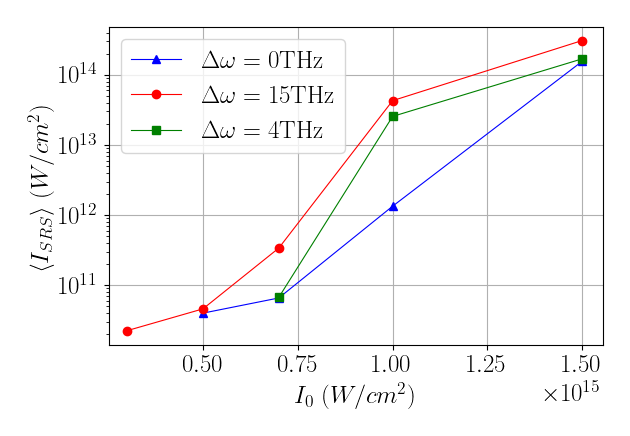
\includegraphics[width=0.75\columnwidth]{Chapters/C5_broadband/fig51_thesis.png}
    \caption{Intensity of light scattered by SRS, averaged over the last three picoseconds of each simulation, for three laser set-ups with fixed maximum normalised chirp ($\Delta\omega \omega_m / \omega_0=5.5\times10^{-6}$) and varied bandwidth. The simulation parameters common to all data-points are: $T_e = 4\si{\kilo eV}; L_n = 400\si{\micro\metre}; n_e(x) = 0.11n_{\text{cr}}\text{exp}(x/L_n);\text{PPC=16,000}. $}
    \label{fig:Wenreplication}
\end{figure}{}


\subsection{Multi-beam SRS}
Studies have also been performed using the code LPSE which show that, at ignition scales, absolute multi-beam backward SRS can be mitigated with bandwidth $\sim 1.6\%$ \citep{Follett2021}.

From this literature review, it is clear that there is no complete picture of how bandwidth affects convective SRS gain in inhomogeneous plasmas.

\section{Decoupled broadband lasers}

The work in this section was presented at the 62nd annual meeting of the American Physical Society Division of Plasma Physics in November 2020.
 
To begin our investigation of the effect of broadband on inflationary SRS, we focussed on the most relevant papers in the literature at the time (\citep{Zhao2019}) This body of work concerns convective SRS in an inhomogeneous plasma, driven by a decoupled broadband laser.


A decoupled broadband laser is defined in Ref \cite{Zhao2017July} as

\begin{equation}\label{eqn:DBL}
  a_{\mathrm{DBL}} = \sum_{i=1}^{N} a_i \mathrm{cos}(\omega_it + \phi_i),
\end{equation}
where $a_i,\omega_i,\phi_i$ are the amplitude, carrier frequency, and phase of
each of the $N$ beamlets. The central frequency and wavelength of the laser is
$(\omega_0,k_0)$ and the total frequency spectrum bandwidth is
$\Delta\omega_0$.

In \cite{Zhao2019} they consider the suppression of parametric
instabilities in a homogeneous plasma by decoupled broadband lasers
(\acrshort{DBL}). 

\subsection{Conclusions}
In conclusion, we decided not to pursue out investigation of DBL-type bandwidth any futher since a) there are no plans to impliment it on lasers of interest and b) 


\section{Realistic laser bandwidth}\label{sec:params}

This section concerns the results of our investigation into broadband suppression of inflationary SRS on different broadband laser systems. The particular form of the broadband may not seem like an important factor to us, but to the EPWs it can be very important.
We consider shock-ignition driven by three different laser systems: frequency-tripled Nd : glass lasers, such as the NIF and LMJ; KrF lasers; and ArF lasers. Each laser has a different frequency and native bandwidth. 

NRL provided us with density, temperatyre and intensity lineouts in 1D from simulations of shock-ignition on these these three laser systems. We selected a single time slice, just before the interaction pulse enters the under-dense plasma created by the assembly pulse. Their simulations were performed using the rad-hydro code \todo{Email and ask what code they used}

\begin{figure}[ht]
   \centering
    \includegraphics[width=\columnwidth]{Chapters/C5_broadband/a_b_c_d_Dens_temp.pdf}
    \caption{Sub-figures a), b), c) show density and temperature line-outs from NRL simulations at the end of the assembly pulse and the start of the ignition pulse. The laser is incident from the right, and the left-hand side boundary represents the quarter critical density surface. The green highlighted areas show the density and temperature range such that $0.3<\kld<0.45$. Sub-figure d) shows the final density and temperature profiles used for our campaign, defined by third order polynomials on the interval $[0,270\si{\micro\metre}]$, and with the laser incident from the left.}
    \label{fig:dens_temp}
\end{figure}{}


For all the simulations presented in this section, the following EPOCH parameters are constant: $\Delta x = \mathrm{min}_x(\lambda_D)$; $\mathrm{PPC} = 2000$; $T_{\mathrm{end}}=6\si{ps}$; thermal boundaries for particles; field boundaries are laser ($x_{\mathrm{min}}$), and absorbing boundaries ($x_{\mathrm{max}}$). We treat the ions as a neutralising background population to allow us to pinpoint the effect of bandwidth on inflationary SRS only. The incident laser intensity is set to be approximately the threshold intensity for inflationary SRS. The threshold intensity is found by varying the intensity for identical PIC set-ups to find the minimum intensity such that the time-averaged intensity of scatter from bSRS is greater than $10\%$ of the incident laser intensity. 

\renewcommand{\arraystretch}{1.25}

\begin{table}[h]\label{tab:laser}
\begin{center}
\begin{tabular}{|l|l|l|l|l|}
\hline
\begin{tabular}[c]{@{}l@{}}Wavelength /\\ nm\end{tabular} & \begin{tabular}[c]{@{}l@{}}Frequency \\ / THz\end{tabular} & \begin{tabular}[c]{@{}l@{}}Intensity / \\ $10^{15}\text{Wcm}^{-2}$\end{tabular} & \begin{tabular}[c]{@{}l@{}}Bandwidth / \\ THz\end{tabular} & \begin{tabular}[c]{@{}l@{}}Bandwidth / \\ $\%$ $\omega_0$\end{tabular} \\ \hline 

351   &  854 &  0.4 to 4.0  &  0, 1, 10 &  0, 0.12, 1.2 \\ \hline

248   & 1209 &   & 0, 3, 6  &  0, 0.25, 0.50   \\ \hline

193   & 1553 & $4\times 10^{15}$   & 0, 5, 8, 10  & 0, 0.32, 0.52, 0.64  \\ \hline
\end{tabular}
\end{center}
\caption{Laser parameters for this investigation. Where multiple values are presented in a list, each represents a different simulation. The incident laser intensity is set to be approximately the threshold intensity for inflationary SRS. The choice of bandwidths and their implementations in EPOCH are explained and referenced in Sections \ref{sec:351}, \ref{sec:248}, \ref{sec:193}, for the 351, 248, 193 nm cases respectively.}
\end{table}


\renewcommand{\arraystretch}{1.25}
\begin{table}[h]
\begin{center}
\begin{tabular}{|l|l|l|l|l|l|}
\hline
Wavelength / nm & $L_x$ /$\si{\micro\metre}$ & $T_e$ / keV & $n_e$ / $n_{cr}$ & $\omega_{pe}$ / $\omega_0$ & $L_n$ / $\si{\micro\metre}$
\\ \hline 
351 & 270 & 5.4 & $[0.105,0.175]$ & $[0.33,0.42]$ & $[420,590]$ \\ \hline
248 & 270 & 3.4 & $[0.078,0.137]$ & $[0.27,0.38]$ & $[400,550]$ \\ \hline
193 & 275 & 3.5 & $[0.071,0.140]$ & $[0.26,0.37]$ & $[330,470]$ \\ \hline
\end{tabular}
\end{center}
\caption{Table shows plasma parameters from simulations performed at the NRL, chosen such that $\kld$ is between 0.3 and 0.45. The temperature given is the maximum temperature of the particles initialised at $t=0$, as there is, in reality, a slight temperature gradient in the electron profile.}
\label{tab:plasma}
\end{table}

\renewcommand{\arraystretch}{1.25}
\begin{table}[h]
\begin{center}
\begin{tabular}{|l|l|l|l|l|l|}
\hline
$\lambda_0$ / nm & $n_e$ or $T_e$ & $a_0$ & $a_1$ & $a_2$ & $a_3$
\\ \hline 
351 & density & $1.05 \times 10^{-1}$  & $1.81 \times 10^2$ & $2.02 \times 10^5$ & $6.47 \times 10^8$ \\ \hline
351 & temperature & $5.28$ & $3.16 \times 10^2$ & $6.60 \times 10^5$ & $1.80\times 10^8$ \\ \hline
248 & density & $8.21 \times 10^{-2}$ & $1.52 \times 10^2$ & $2.46 \times 10^5$ & $3.55\times 10^8$  \\ \hline
248 & temperature & $3.58$ & $9.50 \times 10^2$ & $1.42\times 10^6$ & $-1.27 \times 10^9$ \\ \hline
 193 & density & $7.06\times 10^{-2}$ & $1.66\times 10^2$ & $3.95\times 10^4$ & $1.01\times 10^9$\\ \hline
 193 & temperature & $3.01$ & $1.47 \times 10^3$ & $1.31\times 10^6$ & $-2.27\times 10^9$ \\ \hline
\end{tabular}
\end{center}
\caption{Just trying to put in the coefficients somehow (193: $x_{max}$ = 272 microns) (248: $x_{max}$ = 271microns)}
\label{tab:coeffs}
\end{table}

\section{351nm Nd : glass laser}\label{sec:351}

\begin{figure}[ht]
   \centering
    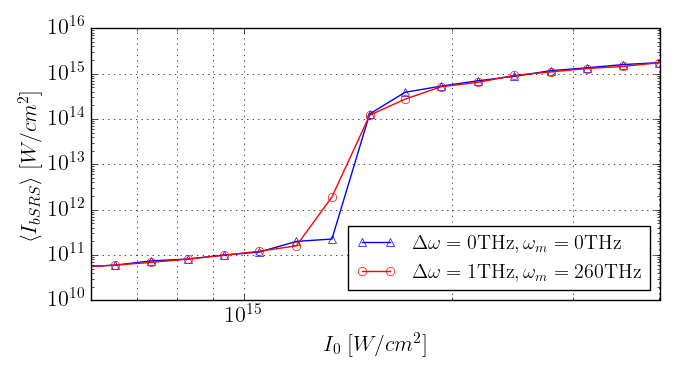
\includegraphics[width=\columnwidth]{Chapters/C5_broadband/351nm_delw1_delw0.png}
    \caption{Intensity of light scattered by backward SRS, time-averaged for all $t>2\si{ps}$. The incident laser intensity varies between $4\times10^{14}\si{W/cm^2}$ and $4\times10^{15}\si{W/cm^2}$.}
    \label{fig:351nm_base_threshold}
\end{figure}{}


\subsection{Base case: $\Delta f=0$}
As stated in Section \ref{sec:params}, the plasma density and temperature profiles are taken from the library of radiation hydrodynamic simulations at the Naval Research Laboratory. 

Sorry this is a horrible way to write this, but this is the detailed plasma set-up: $T_e(x) = \sum^3_{i=0} T_i x^i$, $n_e(x) = n_{\mathrm{cr}}\sum^3_{i=0} n_i x^i $;
$\{T\}_i  = \{3.01, 1.47\times10^3,1.31\times10^6,-2.27\times10^9\}$;
$\{n\}_i  = \{0.07, 165, 3.95\times10^4, 1.01\times10^9\}$. 



\subsection{SSD-type bandwidth: $\Delta f=1\si{THz}$}
1THz is the maximum bandwidth currently implemented by SSD on a 351nm laser, achieved at the Omega laser facility \citep{Regan2005}. According to \citet{Wen2021}, in order to increase the iSRS threshold we require that the modulation frequency satisfies $\omega_m \gg \omega_{pe} c / 2L_n\Delta\omega$. From the plasma parameters given in Table \ref{tab:plasma} and bandwidth of 1THz, this requirement becomes: $\omega_m \gg 128  \si{THz}$. This is problematic, since the optimal modulation frequency for SSD-type smoothing is on the order of $10 \si{GHz} = 0.001 \si{THz}$ \citep{Regan2005,Kelly2013}.

We can implement a continuous-bandwidth frequency-modulated laser in EPOCH using the standard EPOCH laser-driver like so:

\begin{equation}
\begin{aligned}
   E(x,t) &= E_0\text{sin}\left(\omega_0 t - \phi(x,t)\right) \\
   \phi(x,t) &= \frac{1}{2}\frac{\Delta\omega}{\omega_m}\text{sin}\left(\omega_mt - \frac{\omega_m}{c}x\right).
\end{aligned}
\end{equation}

\subsection{Optical parametric amplification: $\Delta f=10\si{THz}$}
According to \citet{Lehmberg2020} ``Parametric amplification may allow bandwidths up to 10 THz from 351 nm glass systems...".


\begin{figure}[ht]
   \centering
    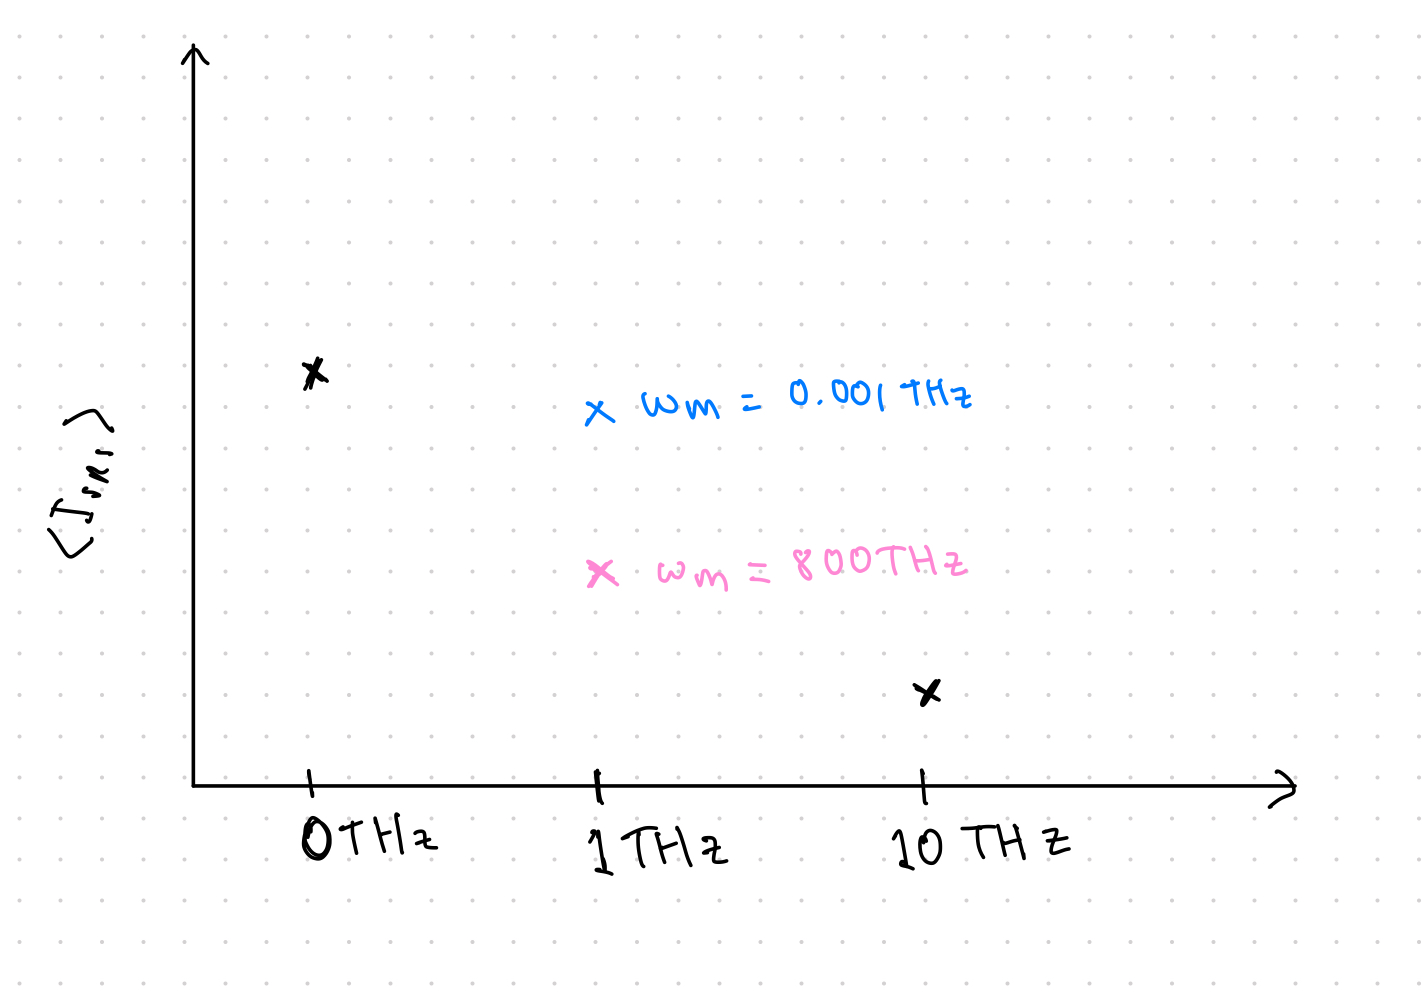
\includegraphics[width=0.75\columnwidth]{Chapters/C5_broadband/ndglass_placeholder.jpeg}
    \caption{placeholder figure for Nd glass sim results}
    \label{fig:NdGlass}
\end{figure}{}

\section{248nm krypton fluoride}\label{sec:248}

\subsection{Base case: $\Delta f=0$}




\subsection{Intrinsic bandwidth: $\Delta f=1,2,3$ $\si{THz}$}
Intrinsic bandwidth of KrF laser such as Nike is predicted to be 3Thz \citep{Obenschain15}

\subsection{Self phase modulation: $\Delta f=4,5,6$ $\si{THz}$}

According to this paper: "Stimulated rotational Raman scattering of arbitrarily polarized broadband light" \citep{Lehmberg2020} the SPM bandwidth of KrF limited to 6THz cos of physics.

\section{193nm argon fluoride}\label{sec:193}
Excimer lasers have a broad amplification spectrum in the UV when compared to Nd: glass lasers. In this section we consider the argon fluoride (ArF) laser under development at the NRL, which is predicted to have native bandwidth up to 10THz \citep{Obenschain2020}.

\subsection{Base case: $\Delta f=0$}



\subsection{Intrinsic bandwidth: $\Delta f =5,8,10$ $\si{THz}$}
In this section, we perform a series of simulations at different bandwidths which are considered realistic for ArF laser systems currently under development \citep{Obenschain2020}. To model the continuous laser spectrum, we follow the method presented in \citet{Bates2020} and distribute 50 beamlets of different frequencies around the central frequency. The intensities of the lines follow a Gaussian distribution whose FWHM is given by the laser bandwidth. \citet{Follett2019} says 50 is enough for a gaussian beam up to 10 percent. Each beamlet has a random phase so the total driven laser field looks like this:



\begin{equation}
\begin{aligned}
	E(x,t) &= \sum_{i=1}^{50} E_i \mathrm{sin}(\omega_i t + \phi_i) \\
	\phi_i & \in  [0,2\pi] \\
	\omega_i & \in [\omega_0 - \Delta\omega / 2, \omega_0 + \Delta\omega / 2]
\end{aligned}
\end{equation}

\begin{figure}[ht]
   \centering
    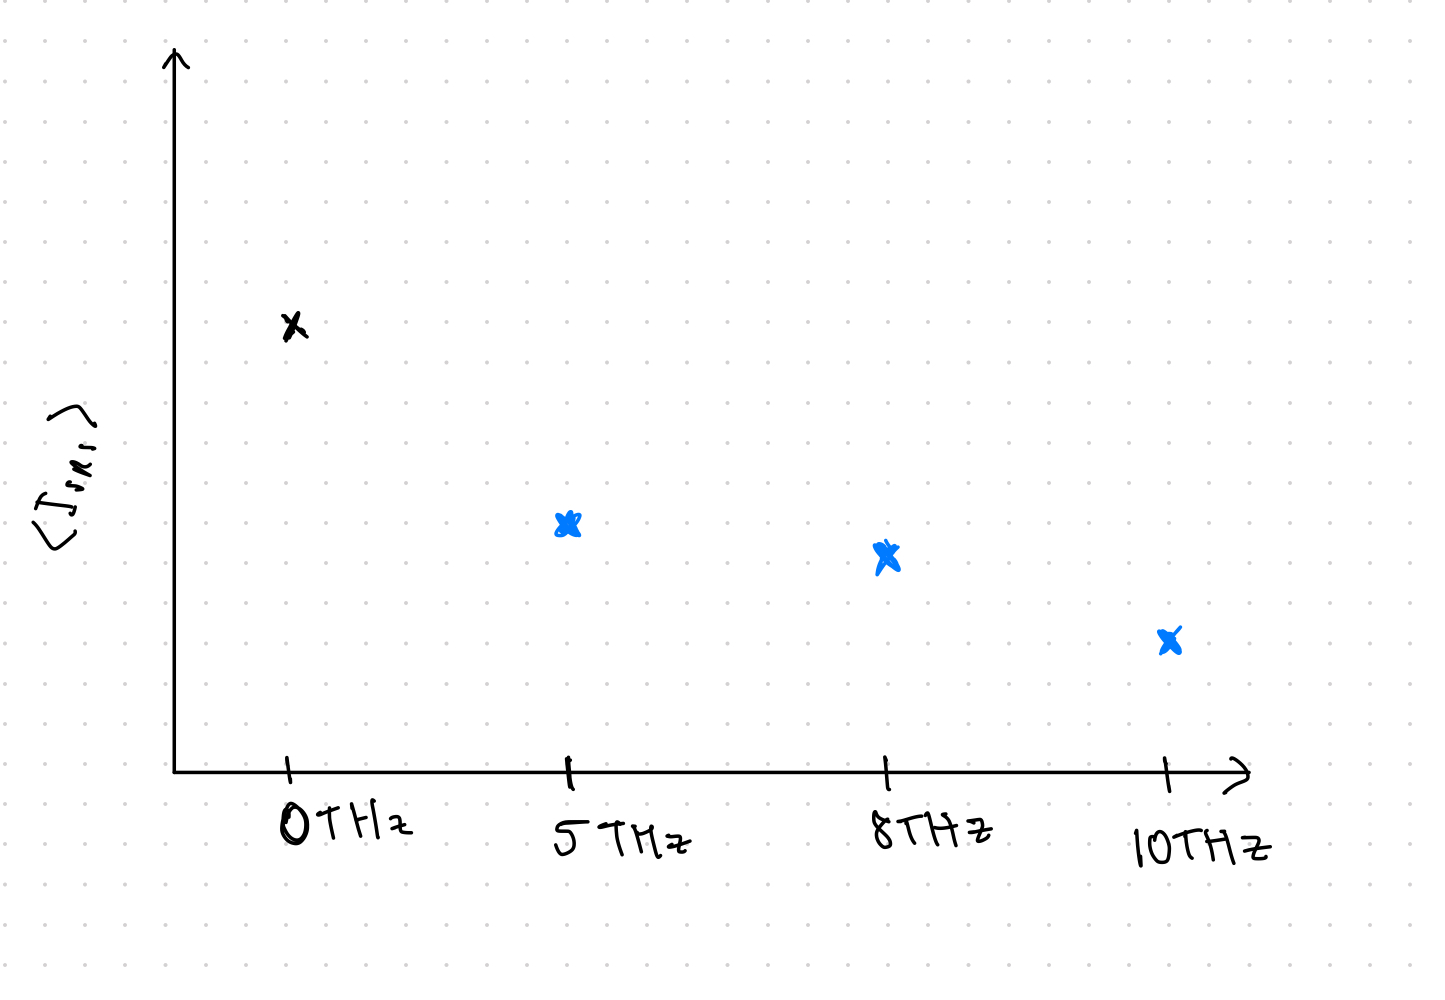
\includegraphics[width=0.75\columnwidth]{Chapters/C5_broadband/arf_placeholder.jpeg}
    \caption{placeholder figure for ArF sim results}
    \label{fig:ArF}
\end{figure}{}


\section{Conclusion}


%\bibliographystyle{plainnat}
%\bibliography{Chapters/C5_broadband/broadband}
